% please generate pdf with the pdflatex command
\documentclass[a4paper,12pt]{article}

\usepackage{graphicx}
\usepackage[brazilian]{babel}
\usepackage[utf8]{inputenc}
\usepackage{fancyhdr}
\usepackage{hyperref}

\hypersetup{bookmarks=true, unicode=true, pdftoolbar=true, pdfmenubar=true, pdffitwindow=true}

\pagestyle{fancy}
\renewcommand{\headrulewidth}{0.0pt}
\renewcommand{\footrulewidth}{0.0pt}
\fancyhead{}
\fancyhead[C]{versão 0.32}

% \setlength{\parindent}{0pt}
% \setlength{\parskip}{\baselineskip}

\def\blog{\emph{CMS}}
\def\feeds{\emph{RSS}}
\def\plugin{\emph{plugin}}
\def\queue{\emph{Queue}}
\def\url{\emph{URL}}
\def\dragndrop{\emph{drag and drop}}

% links
\def\gerenciadorconteudo{\hyperref[gerenciadorconteudo]{gerenciador de conteúdo}}
\def\tipoblog{\hyperref[tipoblog]{tipo de \blog{}}}
\def\dialogovisualizacao{\hyperref[dialogovisualizacao]{diálogo de visualização}}
\def\metodoalimentacao{\hyperref[metodoalimentacao]{método de alimentação}}
\def\metodopublicacao{\hyperref[metodopublicacao]{método de publicação}}
\def\dialogopublicacao{\hyperref[dialogopublicacao]{diálogo de publicação}}
\def\gerenciadorpublicacao{\hyperref[gerenciadorpublicacao]{gerenciador de publicação}}

\begin{document}

\title{Software para integração de \emph{feeds} e sistemas de gerenciamento de conteúdo}
\author{Marcelo Toledo \and Rafael Castilho}
\date{\today}

\maketitle

\newpage
\section{Introdução}

\paragraph{}
Sistemas de gerenciamento de conteúdo (CMS), em particular os populares
\emph{blogs}, são ferramentas que permitem a publicação de conteúdo em um
endereço \emph{WEB}, e que exigem apenas o conhecimento do uso da
\emph{interface}.

\paragraph{}
Em geral, os \blog{}s permitem a visualização de itens de conteúdo publicado na
forma parametrizada \feeds{} por meio de canais alimentadores (\emph{feeds}). Uma
das ferramentas mais utilizadas pelos \emph{blogueiros} é o agregador de
\feeds{}, capaz de coletar e organizar o conteúdo de diversos canais
simultaneamente.

\paragraph{}
Em um \emph{blog}, além de conteúdo próprio, é comum a citação de conteúdo de
terceiros, realizado de forma "artesanal", através da cópia das informações
disponíveis na página \emph{WEB} ou no agregador e da colagem no editor de
publicação do \blog{}.

\paragraph{}
O objetivo do software a ser desenvolvido é disponibilizar um agregador de
canais que permita a publicação de itens de conteúdo no \blog{} do cliente de
forma ágil, padronizada, e com base em suas preferências.

\section{Especificação funcional}

\paragraph{}
Esta especificação funcional tem como objetivo detalhar o funcionamento da
aplicação, sem detalhar questões de usabilidade.

\subsection{Cadastro de perfil de acesso}

\paragraph{}
Para ter acesso ao software, o cliente deve efetuar a autenticação de um perfil
de acesso a partir de um endereço de e-mail e senha cadastrados.

\subsubsection{Novo perfil}

\paragraph{}
O cadastro de um novo perfil de acesso é feito a partir do formulário de
autenticação, através da opção "não cadastrado", que quando acionada, passa a
exibir o formulário para um novo cadastro. 

\begin{center}
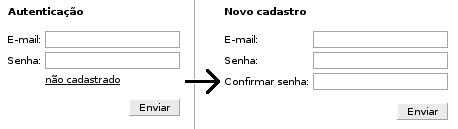
\includegraphics[scale=0.8]{authform.png}
\end{center}

\paragraph{}
O procedimento para criação de um novo perfil a partir do formulário para um
novo cadastro deve ser feito como segue:

\begin{enumerate}
\item Informar um endereço de e-mail, senha e confirmação de senha;
\item Se o endereço de e-mail não estiver cadastrado em um perfil de acesso, o
cliente deverá receber uma mensagem de e-mail contendo uma \url{} de
confirmação de cadastro;
\item Após a confirmação de cadastro, o cliente deverá reber uma mensagem de
e-mail contendo uma notificação de cadastro confirmado e instruções para o
primeiro acesso.
\item Se o endereço de e-mail informado já estiver cadastrado, o cliente deverá
receber uma mensagem de e-mail contendo uma notificação da existência do perfil
com instruções para acesso e alteração de senha (se necessário).
\end{enumerate}

\subsubsection{Atualização de perfil}

\paragraph{}
Após efetuar o acesso, o cliente poderá alterar suas informações de acesso,
preencher seus dados pessoais (nome, país, região, cidade, distrito, endereço,
código postal, etc.), informar seu idioma, etc.

\paragraph{}
Para alteração do endereço de e-mail, o cliente deverá efetuar o seguinte
procedimento:

\begin{enumerate}

\item Acionar o comando de alteração de endereço de e-mail, que enviará uma
mensagem ao endereço atual com instruções para alteração.

\item A mensagem deve conter uma \url{} que permite acesso ao formulário de
alteração de endereço de e-mail, onde o cliente deve informar o novo endereço.

\item Uma mensagem deve ser enviada ao antigo e novo endereços notificando a
alteração.

\end{enumerate}

\subsubsection{Recuperação de acesso}

\paragraph{}
O software deve permitir ao cliente recuperar o acesso quando não recordar sua
senha, através do seguinte procedimento:

\begin{enumerate}

\item Informar o endereço de e-mail do perfil de acesso;

\item Se o endereço de e-mail estiver cadastrado em um perfil de acesso, o
cliente receberá uma mensagem de e-mail com uma \url{} para o formulário de
alteração de senha;

\item O formulário de alteração de senha deve permitir ao cliente digitar uma
nova senha. Após a alteração, o software deverá enviar uma mensagem de e-mail
ao cliente com a notificação de alteração.

\item Se o endereço de e-mail informado não estiver associado a um perfil de
acesso, o cliente deverá receber uma mensagem de e-mail com a notificação da
não existência do perfil de acesso e instruções para a criação de um novo.

\end{enumerate}

\subsection{Cadastro de \blog{}}

\subsubsection{Novo \blog{}}

\paragraph{}
Após efetuar acesso, o cliente poderá realizar o cadastro de um novo \blog{}
através das seguintes etapas:

\begin{enumerate}

\item Informar o nome do \blog{};

\item Informar a \url{} raiz do \blog{}. O software deverá detectar o \tipoblog{}
(\emph{Wordpress}, \emph{Joomla}, \emph{Drupal}, etc.) a partir da \url{}
informada;

\item Se for possível a detecção do tipo de \blog{}, o software deverá verificar
a existência do gerenciador de publicações do \blog{} em um endereço padrão, de
acordo com o tipo de \blog{} e da \url{} raiz;

\item Se o gerenciador de publicações do \blog{} não estiver disponível no
endereço padrão, permitir que o cliente informe seu endereço através de uma
\url{}. O software deverá verificar se o endereço informado é válido como
gerenciador de publicações para o tipo de \blog{} escolhido;

\item Se a detecção do tipo de \blog{} não for bem sucedida, verificar a causa e
informar o erro mais provável (endereço ou página não encontrados, erro no
servidor, etc.);

\item Se o endereço estiver correto mas o tipo não for suportado, exibir
notificação ao cliente e informar os tipos suportados. Permitir também que o
cliente digite o tipo utilizado. Neste caso, o cadastro de \blog{} é descontinuado;

\item Após a determinação correta do tipo de \blog{} e endereço do gerenciador
de publicações, solicitar ao cliente que informe o usuário e senha do
gerenciador. O software deverá verificar se o usuário e senha permitem
autenticação no gerenciador, caso contrário, notificar ao cliente que o usuário
e senha não são válidos;

\item O software deve verificar de forma não invasiva (sem publicar conteúdo em
produção) se o acesso ao gerenciador de publicações possui permissão para
escrita de conteúdo (ex. \emph{drafts} do \emph{Wordpress}). Se não for
possível tal verificação, o software poderá solicitar ao cliente se deseja
realizar um teste de publicação em produção.

\end{enumerate}

\subsection{Cadastro de canal \feeds{}}

\paragraph{}
O cadastro de canais \feeds{} deverá pertencer a um \blog{} já cadastrado.

\paragraph{}
Para adicionar um novo canal, o cliente deve informar a \url{} do alimentador
ou um arquivo de importação \emph{OPML}.

\paragraph{}
O título de um novo canal é definido pelo \gerenciadorconteudo{}.
Posteriormente o cliente poderá informar o título de sua preferência.

\paragraph{}
Durante a importação de canais em um arquivo \emph{OPML}, o título do canal
será o mesmo definido no arquivo de importação.

\subsection{\emph{Dashboard}}

\paragraph{}
O \emph{dashboard} é a visualização padrão após a autenticação, composto por
diversos painéis que permitem o gerenciamento das informações. 

\begin{center}
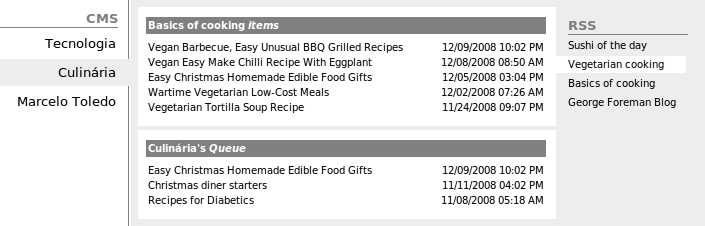
\includegraphics[scale=0.5]{dashboard.png}
\end{center}

\subsubsection{Painel de \blog{}}

\paragraph{}
O painel de \blog{} contém a lista de \blog{}s cadastrados. A exibição das informações nos demais painéis depende do \blog{} selecionado.

\subsubsection{Painel de canais \feeds{}}

\paragraph{}
O painel de \feeds{} contém a lista de canais \feeds{} cadastrados para o \blog{}
selecionado.

% definir a relevância do conteúdo através da ordem dos canais. isto é
% realmente necessário?
% \paragraph{}
% A ordem de um canal em relação aos demais determina a sua relevância. Quanto
% mais no topo, maior relevância.

\paragraph{}
Novos canais são adicionados ao final da lista. Deve ser possível determinar a
ordem dos canais através de \dragndrop{} ou por ordem alfabética.

\paragraph{}
Um canal deve poder ser desativado ou removido. 

\subsubsection{Painel de itens de conteúdo}

\paragraph{}
O painel de itens de conteúdo exibe a lista de itens de todos os canais ativos.
Quando um canal é selecionado, exibe apenas os itens do respectivo canal.

\paragraph{}
O cliente poderá determinar a quantidade $n$ de itens que devem aparecer na
lista por vez. Serão carregados os últimos $n$ itens a partir da data de
publicação em ordem decrescente.

\paragraph{}
A relevância de um item de conteúdo é obtida através do número de vezes em que
o item é publicado, envolvendo a estatística de todos os clientes que utilizam
o software. Deve ser exibido na forma de um indicador no item.

\paragraph{}
Um item poderá ser marcado com uma estrela, para que possa ser filtrado
posteriormente pelo \metodoalimentacao{}.

\paragraph{}
Para visualizar um item, o cliente deve acionar o comando "visualizar", que
exibirá o \dialogovisualizacao{}.

\paragraph{}
Um item pode ser adicionado ao \queue{} através de \dragndrop{} ou através do
comando "adicionar ao \queue{}". Um marcador deve indicar quando um item deste
painel encontra-se disponível no painel de \queue{}.

\paragraph{}
O método de alimentação define as regras de automação na adição de itens deste
painel ao painel de \queue{}.

\subsubsection{Painel de \queue{}}

\paragraph{}
O painel de \queue{} contém a lista de itens de conteúdo selecionados para
publicação.

\paragraph{}
A publicação de itens manualmente é feita através do \dialogopublicacao{},
acionado pelo cliente através da seleção de um item do \queue{} e do comando
"abrir diálogo de publicação".

\paragraph{}
Novos itens são adicionados ao final da lista. A ordem dos itens pode ser
alterada através de \dragndrop{}.

\paragraph{}
O \metodopublicacao{} define as regras de automação na publicação de conteúdo
no \blog{}.

\subsubsection{Diálogo de visualização} \label{dialogovisualizacao}

\paragraph{}
O diálogo de visualização exibe todas as informações disponíveis para um item
de conteúdo (título, data de publicação, fonte, etc.), além de um \emph{link}
para visualização do conteúdo no endereço de origem.

\subsubsection{Método de alimentação} \label{metodoalimentacao}

\paragraph{}
O método de alimentação é um conjunto de configurações que determinam a forma
como um item da lista de itens de conteúdo é adicionado ao painel de \queue{}.

\paragraph{}
A primeira configuração define o estado de alimentação, que pode assumir os
valores "manual" ou "automático". No estado manual, os itens de conteúdo são
adicionados ao \queue{} somente através da ação do cliente.

\paragraph{}
O estado automático atribui ao software a responsabilidade na adição de itens
ao \queue{}, e para isso, solicita ao cliente as seguintes configurações:

\begin{itemize}

\item Com estrela: Somente itens marcados com estrela no painel de itens de
conteúdo serão utilizados para adição. Padrão: Todos;

\item Palavras-chave: A escolha de itens é feita com base em uma ou mais
palavras-chave. Padrão: Em branco;

\item Ordenação: Define a ordem de adição de itens a partir da data de
publicação, relevância ou randômico. Padrão: Data de publicação;

\item Máximo: Quantidade máxima de itens que podem ser adicionados ao \queue{}.
Enquanto o número de itens do \queue{} não for menor ou igual ao número de
itens definido por esta configuração, novos itens não poderão ser adicionados
ao \queue{}. Padrão: 5 itens. Máximo: 25 itens;

\end{itemize}

\paragraph{}
A adição de itens ao \queue{} manualmente sempre deve estar disponível, sem
considerar as configurações de estado.

\subsubsection{Método de publicação} \label{metodopublicacao}

\paragraph{}
O método de publicação é um conjunto de configurações que determinam a forma
como um item de conteúdo do painel de \queue{} é publicado no \blog{}.

\paragraph{}
De forma análoga ao método de alimentação, o método de publicação pode assumir
os valores de estado "manual" ou "automático". No estado manual, um item
somente é publicado através da ação do cliente.

\paragraph{}
O estado automático atribui ao software a responsabilidade na publicação de
itens no \blog{}, e para isso, solicita ao cliente as seguintes configurações:

\begin{itemize}

\item Frequência: Define o intervalo de tempo entre as publicações (ex: 5min
15min, 30min, 1hora, 2hrs, 3hrs, 6hrs, 12hrs, 24hrs). Padrão: 30min;

\end{itemize}

\paragraph{}
No estado automático, a ordem dos itens no \queue{} determina a ordem de
publicação. Os itens do início da lista são publicados em primeiro.

\paragraph{}
A publicação de itens no estado automático é gerenciada pelo \gerenciadorpublicacao{}.

\paragraph{}
A publicação de itens ao \queue{} manualmente sempre deve estar disponível, sem
considerar as configurações de estado.

\subsubsection{Diálogo de publicação} \label{dialogopublicacao}

\paragraph{}
O diálogo de publicação exibe as informações de um item de conteúdo (título,
data de publicação, fonte, etc.) e permite a alteração dos valores, além de um
campo para comentários adicionais.

\paragraph{}
Deve estar disponível uma opção para indicar a fonte do conteúdo, que quando
selecionada, inclui no final do conteúdo un \emph{link} para a notícia no
endereço de origem.

\paragraph{}
A publicação do conteúdo é feita através do comando "publicar".

\paragraph{}
É possível armazenar as alterações feitas em um item através do comando
"salvar", sem necessariamente publicá-lo.

\paragraph{}
Informações adicionais podem ser incluídas na publicação de conteúdo
(Categorias, \emph{Tags}, etc.), dependendo somente da implementação
dos recursos necessários no \plugin{} do tipo de \blog{} utilizado. 

\subsection{\emph{Back-end}}

\paragraph{}
O \emph{back-end} é o conjunto de ferramentas do software responsável por
gerenciar os recursos de forma independente ao cliente.

\subsubsection{Tipo de \blog{}} \label{tipoblog}

\paragraph{}
O tipo de \blog{} define qual software é utilizado pelo cliente. Os tipos
disponíveis serão adicionados ao software na forma de \emph{plugins}, e devem
implementar uma interface determinada pelo software.

% TODO: definir os métodos da interface de plugins

\paragraph{}
Um \emph{plugin} de \blog{} deve ser capaz de gerenciar as diferentes versões de
um tipo de \blog{}.

\subsubsection{Gerenciador de conteúdo} \label{gerenciadorconteudo}

\paragraph{}
Os itens de conteúdo de um canal podem ser compartilhados por todos os
clientees do software, afim de eliminar redundância desnecessária de
informações.

\paragraph{}
Quando um novo canal é adicionado, o sistema obtém as informações sobre o canal
(título, descrição, etc.) e os itens de conteúdo disponíveis.

\paragraph{}
Um \emph{daemon} deverá obter novos itens de conteúdo para um canal cadastrado,
com uma freqüência em função da periodicidade de atualização do conteúdo no
alimentador deste canal.

\subsubsection{Gerenciador de publicação} \label{gerenciadorpublicacao}

\paragraph{}
O gerenciador de publicação possui um \emph{daemon} responsável pela publicação
de conteúdo de um \queue{} em um \blog{} quando o estado do método de publicação
está definido como automático. 

\section{Notas de Implementação}

\paragraph{}
A linguagem escolhida para o desenvolvimento da aplicação foi o \textbf{PHP}. O \emph{core} foi inspirado no \emph{Zend Framework}, que segue uma estrutura no padrão \textbf{MVC}, confirme a seguir:

\begin{itemize}
\item \textbf{application}: arquivos da aplicação no padrão \textbf{MVC};
\subitem \textbf{controller}: controle de ações;
\subitem \textbf{model}: classes de \textbf{ORM};
\subitem \textbf{view}: visualização;
\subitem \textbf{library}: arquivos de biblioteca da aplicação;
\subsubitem \textbf{helper}: \emph{scripts} auxiliares de visualização;
\subsubitem \textbf{layout}: diagramação geral (\emph{layout});
\subsubitem \textbf{template}: diagramação de ações;
\item \textbf{config}: arquivos de configuração;
\item \textbf{db}: arquivos de base de dados (\textbf{SQL});
\item \textbf{library}: arquivos de biblioteca de framework;
\subitem \textbf{AB}: \emph{core} \textbf{MVC};
\subitem \textbf{Zend}: \emph{Zend Framework};
\item \textbf{log}: arquivos de histórico;
\item \textbf{public}: \emph{bootstrap}, deve ser visível para \emph{WEB};
\end{itemize}


\section{Instalação}

\subsection{Ambiente}
O sistema operacional deve ser compatível com \emph{LINUX} ou \emph{UNIX}, deve ter instalado o servidor de \emph{HTTP} \emph{Apache 2} com \emph{mod\_php} e servidor de base de dados não mandatório, porém recomendável, \emph{PostgreSQL}.

\paragraph{}
A configuração do apache deve ser feita de forma semelhante ao exemplo à seguir:

\begin{verbatim}
Listen 127.0.0.1:80
ServerName 127.0.0.1
<VirtualHost 127.0.0.1:80>
    DocumentRoot /var/www/blotomate/public
    <Directory /var/www/blotomate/public>
        AllowOverride All
        allow from all
    </Directory>
    ErrorLog /var/log/apache2/blotomate.error.log
    LogLevel warn
</VirtualHost>
\end{verbatim}

\paragraph{}
Neste caso, a raiz da aplicação encontra-se no diretório \texttt{/var/www/blotomate} e somente a pasta (\emph{DocumentRoot}) \texttt{./public} estará visível para a \emph{WEB}.

\subsection{Zend Framework}

\paragraph{}
A biblioteca \emph{Zend Framework} (\texttt{http://framework.zend.com}) é
pré-requisito para o funcionamento da aplicação. Recomenda-se utilizar a versão
\texttt{1.7}\footnote{http://downloads.zend.com/framework/1.7.3PL1/ZendFramework-1.7.3PL1.tar.gz},
ou verificar a mais recente disponível para \emph{download}:

\begin{verbatim}
$ tar zxvf ZendFramework-1.7.3PL1.tar.gz
$ cd /var/www/blotomate/library
$ ln -s $(pwd)/ZendFramework-1.7.3PL1/library/Zend \
  /var/www/blotomate/library/Zend
\end{verbatim}

\subsection{Configuração}

\paragraph{}
A configuração da aplicação é feita a partir do arquivo
\texttt{./config/environment.php}, onde os seguintes parâmetros deverão ser
ajustados:

\begin{itemize}
\item \textbf{BASE\_PATH}: Localização raiz da aplicação no servidor. \\
Ex: \texttt{/var/www/blotomate};
\item \textbf{BASE\_URL}: Localização raiz da aplicação na rede. \\ 
Ex: \texttt{http://www.blotomate.com/app}, \texttt{http://localhost:80}, etc.;
\item \textbf{database-$>$driver}: \emph{Driver PDO} da base de dados. Padrão:
\texttt{pgsql} (\emph{PostgreSQL}). Para outros drivers, verifique em
\emph{http://br2.php.net/pdo};
\item \textbf{database-$>$host}: Endereço \emph{IP} ou \emph{hostname} do
servidor de base de dados. Ex: \texttt{localhost};
\item \textbf{database-$>$username}: Nome de usuário. Ex: \texttt{postgres};
\item \textbf{database-$>$password}: Senha. (Quando não houver senha, deve
conter o valor do tipo \emph{string} e vazio);
\item \textbf{database-$>$db}: Nome da base de dados. Ex: \texttt{blotomate};
\end{itemize}

\paragraph{}
Todos os caminhos acima devem suprimir o separador "/" no final.

\subsection{Permissões}

\paragraph{}
Deve-se ajustar a permissão dos arquivos abaixo, conforme segue:

\begin{verbatim}
$ chmod a+w ./log/error_log
\end{verbatim}

\subsection{Base de dados}

\paragraph{}
A base de dados deverá estar de acordo com o definido na configuração. Em seguida, deve-se carregá-la com as definições de estrutura e informações padrão:

\begin{verbatim}
$ cd ./db
$ php configure.php schema.sql
$ php configure.php data.sql
\end{verbatim}

\paragraph{}
Caso a utilização do \emph{script} \texttt{configure} acima retorne algum erro, o processo de carga deve ser feita manualmente, respeitando a ordem dos arquivos acima.


\appendix

\section{Observações}

\subsection{\emph{Add-ons}}

\paragraph{}
\emph{Add-ons} são recursos adicionais que podem ser incluídos em versões
futuras, incluídos neste documento apenas como idéias gerais sem a preocupação
de incluir detalhes de implementação.

\paragraph{}
É possível unificar (\emph{merge}) dois ou mais itens do \queue{}. Para isto, é
necessário selecionar os itens correspondentes e acionar o "comando de
unificação de itens", gerando um novo item unificado. Um diálogo deverá ser
exibido solicitando o título deste novo item unificado. Por padrão o título
sugerido é o primeiro item selecionado. O novo item deve conter uma marcação de
unificado. Deve ser possível desfazer a ação através do comando "separar itens
unificados".

\paragraph{}
Quando um tipo de \blog{} não for suportado, e o cliente informar o tipo de
\blog{} utilizado, o \emph{backend} poderá verificar se houve falha na detecção
e solicitar ajuste no desenvolvimento, e informar ao cliente sobre a resolução
do problema. Se o tipo não for suportado, informar ao cliente que o software
não é suportado. É possível também verificar quais são as tendências para
implementações de novos tipos.

\subsection{Segurança}

\paragraph{}
O software deve limitar a quantidade de mensagens de e-mail enviadas durante a
solicitação de um novo cadastro de perfil ou durante a recuperação de acesso a
um perfil de acesso, afim de evitar uso mal intencionado do envio de mensagens.

\paragraph{}
O software deve conter algum tipo de proteção para que as publicações em um
\blog{} não sejam feitas por seu próprio alimentador automaticamente e
indefinidamente (autófago).

\end{document}
